\documentclass[letterpaper]{article}
\usepackage{amssymb}
\usepackage{fullpage}
\usepackage{changepage}
\usepackage{amsmath}
\usepackage{epsfig,float,alltt}
\usepackage{psfrag,xr}
\usepackage[T1]{fontenc}
\usepackage{url}
\usepackage{pdfpages}
\usepackage{epstopdf}
\usepackage[framed,numbered,autolinebreaks,useliterate]{mcode}

%\includepdfset{pagecommand=\thispagestyle{fancy}}
\author{Yi Yang}
\title{EECS 442 Midterm Exam Solution}

\begin{document}
\date{11/01/2016}
\maketitle

\newcommand{\trace}{\mathrm{trace}}
\newcommand{\real}{\mathbb R}  % real numbers  {I\!\!R}
\newcommand{\nat}{\mathbb N}   % Natural numbers {I\!\!N}
\newcommand{\cp}{\mathbb C}    % complex numbers  {I\!\!\!\!C}
\newcommand{\ds}{\displaystyle}
\newcommand{\mf}[2]{\frac{\ds #1}{\ds #2}}
\newcommand{\spanof}[1]{\textrm{span} \{ #1 \}}
\newcommand{\sol}[0]{\textbf{Solution: }}
\newcommand{\pf}[0]{\textbf{Proof:}}
\newcommand{\rme}[0]{\textrm{e}}
\newcommand{\Null}[1]{\textrm{Null}\{#1\}}
\parindent 0pt
%%%%%%%%%%%%%%%%%%%%%%%%%%%%%%%%%%%%%%%%%%%%%%%%%%%%%%%%%%%%%%%%%%%%%%%%%%%%%%%
% Solution for Question 1 begins here - by Yi Yang
%%%%%%%%%%%%%%%%%%%%%%%%%%%%%%%%%%%%%%%%%%%%%%%%%%%%%%%%%%%%%%%%%%%%%%%%%%%%%%%
\section*{Problem 1}
\subsection*{(a)}
We need to show that the result is dependent on the order of rotation. First rotate $\beta$ around y axis, then rotate $\gamma$ around z axis:
$$p' = R_z(\gamma)R_y(\beta)p = 
\begin{bmatrix}
\cos{\gamma} & -\sin{\gamma} & 0\\
\sin{\gamma} & \cos{\gamma} & 0\\
0 & 0 & 1
\end{bmatrix}
\begin{bmatrix}
\cos{\beta} & 0 & \sin{\beta}\\
0 & 1 & 0\\
-\sin{\beta} & 0 & \cos{\beta}
\end{bmatrix}p = 
\begin{bmatrix}
\cos{\beta}\cos{\gamma} & -\sin{\gamma} & \cos{\gamma}\sin{\beta}\\
\cos{\beta}\sin{\gamma} & \cos{\gamma} & \sin{\beta}\sin{\gamma}\\
-\sin{\beta} & 0 & \cos{\beta}
\end{bmatrix}
p
$$
If we first rotate $\gamma$ around z axis and then rotate $\beta$ around y axis, we can get:
$$p' = R_y(\beta)R_z(\gamma)p = 
\begin{bmatrix}
\cos{\beta} & 0 & \sin{\beta}\\
0 & 1 & 0\\
-\sin{\beta} & 0 & \cos{\beta}
\end{bmatrix}
\begin{bmatrix}
\cos{\gamma} & -\sin{\gamma} & 0\\
\sin{\gamma} & \cos{\gamma} & 0\\
0 & 0 & 1
\end{bmatrix}p = 
\begin{bmatrix}
\cos{\beta}\cos{\gamma} & -\cos{\beta}\sin{\gamma} & \sin{\beta}\\
\sin{\gamma} & \cos{\gamma} & 0\\
-\cos{\gamma}\sin{\beta} & \sin{\beta}\sin{\gamma} & \cos{\beta}
\end{bmatrix}
p
$$
Hence, we know these two rotations will produce two different values of $p'$.
\subsection*{(b)}
$$R_x(\alpha)R_y(0)R_z(\gamma) = 
\begin{bmatrix}
1 & 0 & 0\\
0 & \cos{\alpha} & -\sin{\alpha}\\
0 & \sin{\alpha} & \cos{\alpha}
\end{bmatrix}
\begin{bmatrix}
1 & 0 & 0\\
0 & 1 & 0\\
0 & 0 & 1
\end{bmatrix}
\begin{bmatrix}
1 & 0 & 0\\
0 & \cos{\gamma} & -\sin{\gamma}\\
0 & \sin{\gamma} & \cos{\gamma} 
\end{bmatrix}
= 
\begin{bmatrix}
1 & 0 & 0\\
0 & \cos(\alpha + \gamma) & -\sin(\alpha + \gamma)\\
0 & \sin(\alpha + \gamma) & \cos(\alpha + \gamma) 
\end{bmatrix}
$$
We can easily see that the degree of freedom for this rotation is 1 since we can see parameter $(\alpha + \gamma)$ the whole as a parameter.

\section*{Problem 2}
First, we need to prove the homographic transformation H defined as $p' = Hp$ has a form as $KRK^{-1}$. Consider two points $p$ and $p'$ in two images respectively  that corresponds to the same 3D point with world coordinates P. Then we have:
$$p = K[I\; T]P,\quad p' = K[R\; T]P$$
\begin{align*}
p' & = K[R\; T]P\\
   & = KR[I\; T]P\\
   & = KRK^{-1}K[I\; T]P\\
   & = KRK^{-1}p
\end{align*}
Hence, we found that the homographic transformation has a form of $H = KRK^{-1}$.
\subsection*{\underline{Computing H}}
First, let me introduce a brief derivation of DLT algorithm for homographical transformation. For point correspondences located in two images, we have:
$$x_i^\prime = Hx_i\quad x_i^\prime\times Hx_i = 0$$
\begin{align*}
x'\times Hx &= 
\begin{bmatrix}
0 & -x_3' & x_2'\\
x_3' & 0 & -x_2'\\
-x_2' & x_1' & 0
\end{bmatrix}
\begin{bmatrix}
h_1 & h_2 & h_3\\
h_4 & h_5 & h_6\\
h_7 & h_8 & h_9
\end{bmatrix}
\begin{bmatrix}
x_1\\
x_2\\
x_3
\end{bmatrix}\\
&= 
\begin{bmatrix}
-x_1x_3'h_4-x_2x_3'h_5-x_3x_3'h_6+x_1x_2'h_7+x_2x_2'h_8+x_3x_2'h_9\\
x_1x_3'h_1+x_2x_3'h_2+x_3x_3'h_3-x_1x_1'h_7-x_2x_1'h_8-x_3x_1'h_9\\
-x_1x_2'h_1-x_2x_2'h_2-x_3x_2'h_3-x_3x_2'h_3+x_1x_1'h_4+x_2x_1'h_5+x_3x_1'h_6
\end{bmatrix}\\
&=
\begin{bmatrix}
0 & 0 & 0 & -x_1x_3' & -x_2x_3' & -x_3x_3' & x_1x_2' & x_2x_2' & x_3x_2'\\
x_1x_3' & x_2x_3' & x_3x_3' & 0 & 0 & 0 & -x_1x_1' & -x_2x_1' & -x_3x_1'\\
-x_1x_2' & -x_2x_2' & -x_3x_2' & x_1x_1' & x_2x_1' & x_3x_1' & 0 & 0 & 0 
\end{bmatrix}
\begin{bmatrix}
h_1\\
h_2\\
h_3\\
h_4\\
h_5\\
h_6\\
h_7\\
h_8\\
h_9
\end{bmatrix}\\
&= 
Ah
\end{align*}
Let us observe matrix A, we can see that $x_2'\times \text{row 2} + x_1' \times \text{row 1} + \text{row 3} = 0$, we can deduce that rank(A) = 2, which means there exists only 2 independent  equations for each point correspondences. In order to solve H matrix or vector h, we must  provide 4 pairs of point correspondences since the DOF of H is 8. Then we can apply SVD to matrix A to solve for eigenvector matrix and h is represented as the last eigenvector which corresponds to the smallest singular value of A. The estimated matrix H is:
$$H = 
\begin{bmatrix}
-1.8619 & -0.5207 & 591.3803\\
-0.8226 & -2.2354 & 441.5196\\
-0.0044 & -0.0046 & 1.0000
\end{bmatrix}
$$
The Matlab codes for computing H is attached below:
\lstinputlisting[firstline=1, lastline=100]{midterm/Homography.m}
\lstinputlisting[firstline=1, lastline=100]{midterm/q2.m}

\subsection*{\underline{Convolution}}
The Matlab codes for Gaussian blurring is attached below:
\lstinputlisting[firstline=1, lastline=100]{midterm/Gaussian_blurring.m}
The image that is added noise is shown below:
\begin{figure}[H]
\centering
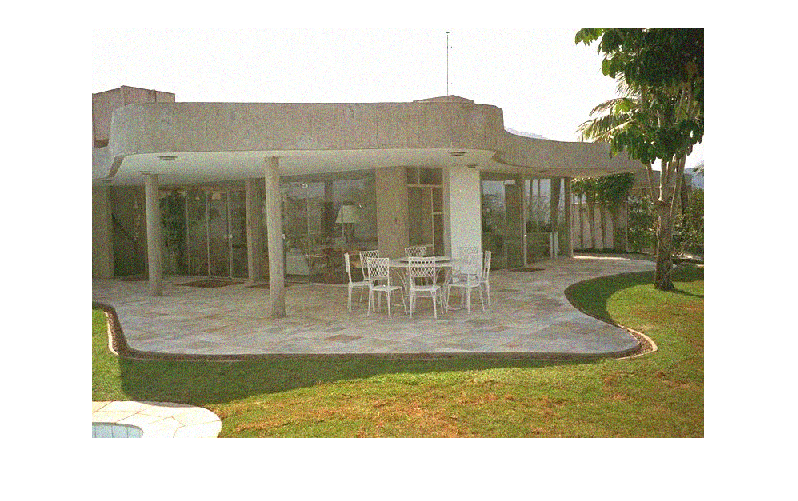
\includegraphics[width=12cm, height=10cm]{midterm/add_noise.png}
\caption{Image with Gaussian White Noise}
\label{noise}
\end{figure}
As shown in figure \ref{noise}, we add Gaussian white noise with mean 0.04 and variance 0.003 to the original image garden1.jpg. Then we design a $9\times 9$ Gaussian kernel with Standard Deviation =1.76 to filter the image and reduce the effects of noise. The filtered image is shown as figure \ref{gaussian}.
\begin{figure}[H]
\centering
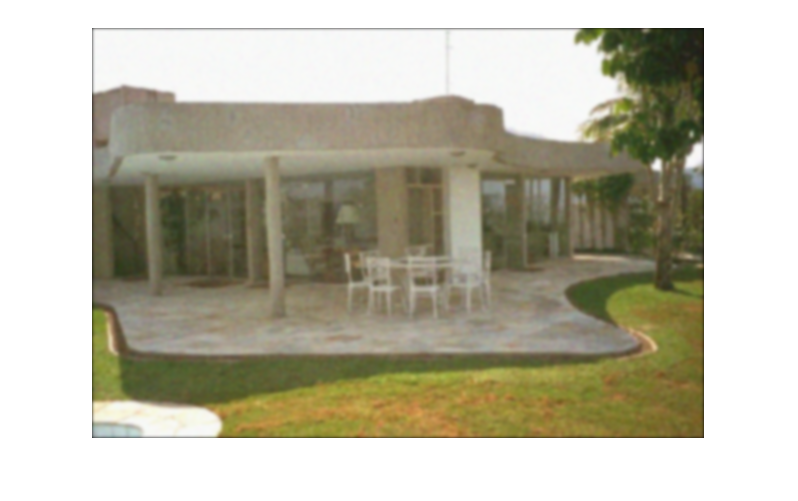
\includegraphics[width=12cm, height=10cm]{midterm/gaussian_blur.png}
\caption{Gaussian Filtering Results}
\label{gaussian}
\end{figure}
\end{document}